%  This LaTeX template is based on T.J. Hitchman's work which is itself based on Dana Ernst's template.
%
% --------------------------------------------------------------
% Skip this stuff, and head down to where it says "Start here"
% --------------------------------------------------------------

\documentclass[12pt]{article}

\usepackage[margin=1in]{geometry}
\usepackage{amsmath,amsthm,amssymb}
\usepackage{graphicx}
\usepackage[UTF8]{ctex}
\usepackage{listings}
\usepackage{cite}
\usepackage{subfigure}
%the following is used for the pseudo-code
\makeatletter
\newif\if@restonecol
\makeatother
\let\algorithm\relax
\let\endalgorithm\relax
\usepackage[linesnumbered,ruled,vlined]{algorithm2e} %[ruled,vlined]{
\usepackage{algpseudocode}
\usepackage{amsmath}
\renewcommand{\algorithmicrequire}{\textbf{Input:}}  % Use Input in the format of Algorithm
\renewcommand{\algorithmicensure}{\textbf{Output:}}  % Use Output in the format of Algorithm \begin{algorithm}


\begin{document}

% --------------------------------------------------------------
%
%                         Start here
%
% --------------------------------------------------------------

\title{计算机视觉的部分基础知识}
\author{王啸峰 from UCAS \& CASIA} % replace with your name

\maketitle

\section{SIFT}
可能的替代:

1. 图像微分:一阶Prewitt、Sobel检测最大值;二阶Laplacian检测过零点。

2. 边缘检测器:Canny:计算梯度、NMS、双阈值提取边缘点、边缘连接。

3. 角点提取:Harris:窗口移动灰度变化,旋转不变,尺度变化。FAST:若灰度比其领域内足够多的像素点的灰度值大或者小。

4. 2D图像的一些变换:投影变换是最大的集合(即单应矩阵)。
\begin{figure}[ht]
    \centering
    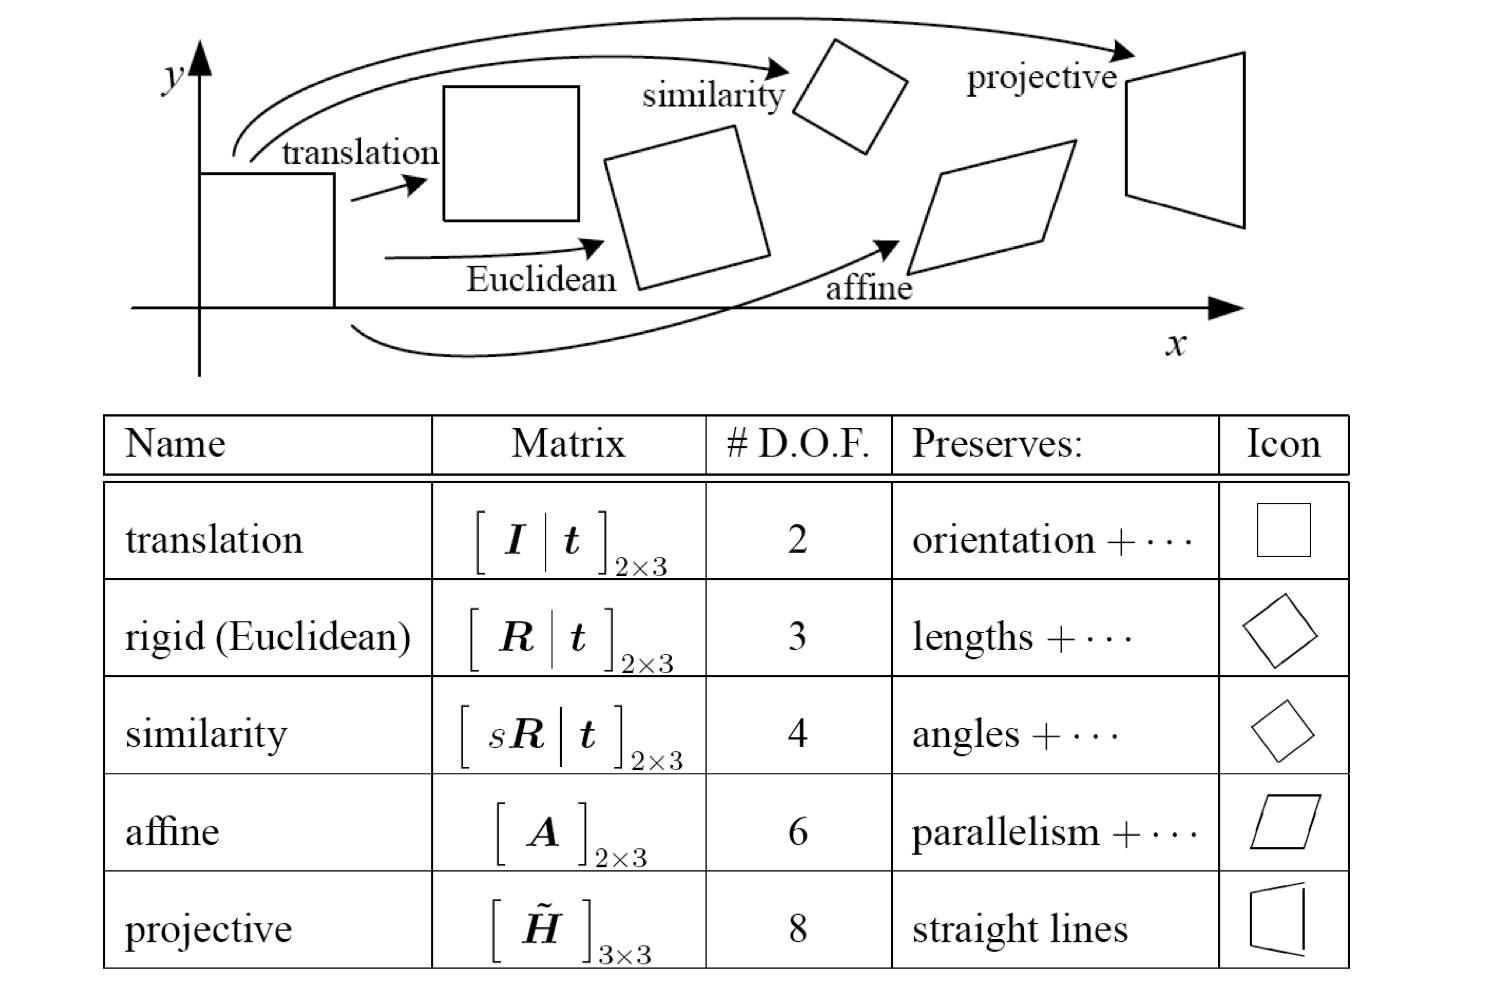
\includegraphics[scale=0.4]{./img/2DTrans.png}
    \caption{2D图像的一些变换}
    \label{fig:2DT}
\end{figure}

SIFT步骤为:多尺度空间(DoG空间)极值点检测,关键点精确定位,关键点主方向计算,描述子构造。
\subsection{特征提取}

1. 多尺度空间(为了在尺度变化时特征稳定):DoG的做法:在同一个分辨率图像上做不同高斯核的模糊后,然后相减;再把这个方法扩展到多分辨率上。
每个分辨率的特征为一个octave下的特征,不同的高斯核相减得到的是在该octave下不同layer的特征。即最后的总特征数为:octave*layer.

2. 极值点检测:检测上述特征的26邻域(3x3x3=27的方块内,减去自己)是否为极值点。

3. 精确定位:上述都是离散采样不够精确,要对DoG进行曲线拟合,即在某一张特征图上进行3维空间的拟合,根据数值分析的方法可以在计算出三维曲面在某一个极值点
的一阶导数和二阶导数,然后一阶导数为0,得到$\Delta X$作为梯度下降的方向,然后逐步收敛到真正的极值点。

4. 去除不稳定的关键点:根据阈值去除对比度低的点;去除边缘点(DoG中边缘点响应强,但是不稳定。)

\subsection{描述子构造}
可能的替代点:ORB:快速,存储低;L2-Net。

希望可以构建一个旋转不变,尺度不变且免除光照影响的描述子。

根据上述DoG的方案获得关键点,已经具有尺度不变了。接下来考虑旋转不变。首先计算关键点的「梯度方向直方图」,即x轴为$(0,2\pi)$,y轴为梯度值的累加。
一般x轴$2\pi$分为10个bins,一个bins36度。然后选取直方图中80\%的bin作为主方向,更精细的方向可以插值得到。也可能有多个主方向。

按关键点的主方向旋转后,再使用双线性插值的方法获取 4x4 个子区域,每个子区域分别计算直方图 (8bins),
直方图的值为梯度值的累加,这样对于每个关键点,我们就有了 4x4x8=128 维的描述子。当然这个也是按照高斯加权,
中间的权重大,附近权重小。

最后把这个描述子按照向量长度进行归一化处理,去除光照的影响(亮度和对比度啥的)。

\subsection{匹配过程}
可能的替代:ICP(Iterated Closest Points):如果知道正确的点对应,那么两个点集之间的相对旋转和平移有闭合解,在ICP中,假设最近的点为对应点;
RANSAC:排除外点。

SIFT匹配策略:NNDR:最近邻距离比率,定义为最近邻距离和次近邻距离的比值。

SIFT搜索策略:BBF:回溯检查总是从优先级最高(best bin)的树结点开始。

\subsection{旋转不变、尺度不变}
尺度不变:DoG;旋转不变:梯度直方图;光照影响:描述子归一化。

\section{Adaboost}

\section{特定方法的分割}
\subsection{Mean Shift}
核心思想:找到概率密度梯度为零的采样点,并以此作为特征空间聚类的中心点。

步骤如下:

1. 在未标记的点中选一个作为中心center;

2. 在一定半径的邻域内,高斯加权后求取新的中心点,然后从原center移动到新的center;

3. 直至移动的shift很小。(即此时的概率密度最高,概率密度梯度为0);

4. shift过程中遇到的所有点都加入此类别,如果此类别的中心和现有类别中心距离很近,则合并为一个类别;

5. 从为遍历过的点中选取一个初始点继续迭代。中途难免会有点既在A类又在B类,那么就看此点出现的频率划分类别。

6. 直至遍历所有的点。

好处就是与K-means相比不需要指定类别个数。缺点是要指定ball-query的半径大小。

\subsection{Ncut:Normalized Cut}
Ncut是图割(graph cut)的升级版本。图割只考虑到了将图划分为两个子集,子集之间的相似度最小(连接权重最小),这样会造成只分割出去一个外点。
Ncut则是考虑到了不仅要子集之间权重低,子集内部的相似性要大。

在Ncut中:

子集之间的相似性度量为两个子集连接边权重之和;

子集i内部的相似性度量为子集i和整个集合的连接边权重之和。(这个定义无法直接表述内部的连接性,但是
我们都是希望这个值越大越好,即如果只有一个外点的话,这个值很小,但是如果集合i的点数比较多,这个值就大。)
\begin{equation}
    \nonumber
    N \operatorname{cut}(A, B)=\frac{\operatorname{cut}(A, B)}{\operatorname{assoc}(A, V)}+\frac{\operatorname{cut}(A, B)}{\operatorname{assoc}(B, V)}
\end{equation}
其中$\operatorname{assoc}(A, V)=\sum_{u \in A, t \in V} w(u, t)$.

但是Ncut是个NP难问题,好在可以构建近似解,具体的步骤是:

1. 给定图像点,构建点集$G(V,E)$,点就是像素点,边权重就是像素距离(如果是RGB就是三维距离)。

2. 求解$(D-W)x=\lambda Dx$的特征值和对应的特征向量。其中$W={w_{ij}}\in\mathbf{R}^{N\times N}$是每个点的相互权重。
$D=diag(d(1),d(2),..., d(N)),\quad d(i)=\sum_jw_{ij}$即每个点和其他所有点的权重之和。

3. 次小特征值和其特征向量进行二分类。

4. 如果需要再分,则在分好的类别中重复上述过程。

\section{CV中的机器学习方法}
\subsection{子空间}
为了处理高维度,非结构化数据。

\subsubsection{主成分分析法PCA}
寻找投影映射P,使得样本从N维降到m 维(m<N),同时最小化重构平方误差。步骤:

1. 计算样本均值$\mu=\frac{1}{n}\sum_{i=1}^{n}x_i$;

2. 计算离散度急诊$S=\sum_{i=1}^{n}\left(x_{i}-\mu\right)\left(x_{i}-\mu\right)^{T}$;

3. 离散度矩阵特征值分解,取前$m$个特征值和特征向量$P\in(N,m)$;

4. 降维$y_i=P^T(x_i-\mu_i)$.

\subsubsection{独立成分分析法ICA}
从多个源信号的线性混合信号中分 离出源信号的技术。假设:源信号统计独立。

\subsubsection{线性判别分析方法LDA}
寻找投影W,使得投影后的样本 类内散度最小,而类间散度最大。

\subsection{流形学习}
上述都是线性的学习方式,但是我们的数据很多都是分线性的,就要从非线性的角度探讨数据的内在几何结构。
\subsubsection{LLE:Locally Linear Embedding}
样本空间与内在低维子空间之间在局部意义下的结构可以用线性空间近似。假设嵌入映射在局部是线性的条件下, 最小化重构误差。
\subsubsection{Isomap等距映射}
之前的版本MDS的基本思想: 约简后低维空间中任意两点间的 距离应该与它们在原始空间中的距离相同.但是光用欧式距离还不能满足,要考虑“测地距离”,也就是Isomap用的方法。

测地距离可以用Dijkstra算法求解。

\subsubsection{Laplacian Eigenmap}
在高维空间中离得很近的点投影到低维空间中的像也应该离得很近。

\subsection{稀疏表达}
上述方法都无需迭代,转换为求解矩阵特征值;并且探讨了数据的非线性结构;都是非参数方法。但是有个问题,在数据稀疏的时候不太好办。

稀疏表达就是想要求解一个问题,给定一堆稠密的数据$D=\left[d_{1}, d_{1}, \ldots, d_{n}\right] \in R^{m \times n}(m \leq n)$,
如何把他们线性组合后来代表一个给定的稀疏点$x=D\alpha$来代表这群稠密数据?其中$\alpha$的非零点越少越好。

这是个NP难问题,但是在RIP(Restricted Isometry Property)条件下,可以转化为凸优化。具体不展开了。
\begin{equation}
    \nonumber
    \begin{array}{l}
        \min _{\alpha}\|\alpha\|_{1} \\
        \text { s.t. }\|x-D \alpha\|_{2}^{2} \leq \varepsilon
        \end{array}
\end{equation}

可以用来做分类问题,比如给定C个类别的图像,然后再给定一张图像要用这C个图像线性组合而成,那么最终求的$\alpha$哪一位的值越大,就是哪一类。


\subsection{低秩表达}
数据矩阵X既包含结构信息,也包含噪声,因此
可以将矩阵X分解为两个矩阵的和,一个是低秩 的,另一个是稀疏的。
% --------------------------------------------------------------
%     You don't have to mess with anything below this line.
% --------------------------------------------------------------

\newpage
\section{附录}

\end{document}